\documentclass[a4paper, 10pt]{article}
\setlength{\topmargin}{-0.8in}
\setlength{\textheight}{9.5in}
\setlength{\oddsidemargin}{-.13in}
\setlength{\textwidth}{6.5in}

\usepackage{multirow}
\usepackage{float}
\usepackage{array}
\newcolumntype{L}{>{\centering\arraybackslash}m{3cm}}

\usepackage{graphicx}
\graphicspath{{images/}}

\begin{document}



\title{User Modeling and Personalisation in Search for People with Autism}
\author{Author: Esha Massand\\Supervisor: Keith Mannock\\
MSc Computer Science Project Proposal\footnote{This proposal is substantially the result of my own work, expressed in my own words, except where explicitly indicated in the text. I give my permission for it to be submitted to the JISC Plagiarism Detection Service. }}
\date{\today}
\maketitle


\begin{abstract}
The current proposal presents my objective to research and build a user model and web application, for individuals on the Autism Spectrum, within Search. The model will be built around the core features of Autism, and applied to search results returned from a synthesis of three leading existing search engines. The web application will also be integrated with motion-controlled user interfaces (UI). The project will provide novel insights into the needs and wants of individuals with Autism within search, and enable future development and interventions within these information streams and communication channels.
\end{abstract}


\tableofcontents

\section{Abbreviations}
\begin{tabular}{l l }
API & Application Programming Interface\\
ASD & Autism Spectrum Disorder\\
DSM & Diagnostic and Statistical Manual\\
GCS & Google Custom Search\\
HCI & Human Computer Interaction\\
JSON & JavaScript Object Notation\\
KWIC & Key Word In Context\\
TDD & Test Driven Development\\
UI & User Interface\\
UX & User Experience\\
VR & Virtual Reality\\
\end{tabular}




\clearpage

\section{Introduction \& Background}
\subsection{Problem Statement} \label{prob}
People with Autism are less context-sensitive and prefer a more detail-focused processing style \cite{mottron}, and they form web-search queries very differently to the typical population. Individuals with Autism are also less likely to engage in a relational (hierarchically organized) style of processing \cite{bowler} suggesting that relating information in a hierarchically organised framework is less likely. Hierarchical organisation implies a great deal of flexibility and mental-shifting, as a simple example, in a search for 'apple', it would imply awareness that the word is related to 'pear' but also to 'fruit'. Awareness of this latter relation also suggests awareness that 'apple' is related to 'pomegranate'. This is of course, a simple example, but these associations can get very complex very quickly. Generally speaking, individuals with Autism prefer, and are more likely to engage in an item-specific processing style, and, whilst intelligent cognition is definitely possible, web-search queries are more likely formed of first-order associations\footnote{Of course there is a great deal of individual variability in the Autism Spectrum.}.To address this issue, the current project aims to build a user model within Search for individuals with Autism. 

\subsection{The Role of Context Within Search} \label{the problem}
It is unlikely that any given page on the web will contain a word or phrase that means exactly (or nearly) the same as another word or phrase in that language (e.g., shut and close). How is it then that your search engine picks these phrases to mean the same thing, and returns them synonymously in the results of your query? Well, quite simply put, it is by virtue of the fact that each of their neighbouring words and associations are similar. These are indirect, higher-order associations, and provide the context in which the search engine index keywords.

Most search engines apply user models to refine user search queries. These models can often lack specificity for users/groups of users \cite{usermodel}. Although adaptive search engines have now become prominent (using search history, locale, and demographics to guess the user's intentions) these models make several a priori assumptions about users from specific subgroups. Based on the Psychology literature, general user models and the needs of the user with Autism differ. Despite Autism being amongst the most common neurodevelopmental condition (1/68 children meet criteria for Autism Spectrum \cite{CDC}), no user model has yet been developed for Autism. 

According to the Diagnostic and Statistical Manual (2013), Autism is characterized by persistent and early deficits in reciprocal social interaction, so interaction with computers is prominent in this group. It is also well established that individuals with Autism are more engaged when using technology that is receptive and interactive (e.g., games, responsive consoles, motion controlled devices) compared to technology that is not \cite{motioncontrollerforautism}, this project will combine interactive, motion recognition hardware with Search to also improve the UI (user interface) of Search for individuals with Autism.

\subsection{The Downfalls of Current Search Tools for People with Autism}\label{What should Search offer people with Autism}

The Internet is one of the largest resources of information. Search engines allow users to collate hundreds of links on a single topic, using only a few words or phrases. The typical user sorts the returned results into 'relevant' or 'irrelevant' categories, flexibly shifting (mentally) between one result and the next, to determine the relevance of each page returned by the search engine. Search allows the user to assimilate the information on the page into their knowledge and is an important learning tool. For people with Autism, the requirement is no different; search is an important tool for learning. However, current search is not adequate because the requirement to 'mentally shift' between results is far harder for people with Autism \cite{disengagement}. The information is therefore harder to assimilate and learn for them. 

Individuals with Autism have poor attention \cite{attention}. The static 2-dimensional interface of many current search engines are unlikely to maintain adequate (sustained) interest levels. Individuals (and especially teenagers) with Autism spend a substantial amount of their time using computers, web, portable or console devices \cite{Shane and Albert}, as they find these more stimulating and attention-grabbing. For these individuals, computer-based technologies provide a stable, consistent learning environment that can be customized \cite{moore}. Furthermore, motion recognition devices can be programmed to make consistent responses to environmental triggers. These controlled and interactive environments have shown promise for improving social communication skills and reducing repetitive behaviours \cite{gameshealth}. For the current project a motion-controlled learning environment will be bolstered to improve attention within search for people with autism. 

Current search is text-ridden and extremely verbal. People with Autism demonstrate stronger visual memory \cite{fabienne} than verbal memory, so a more visually-oriented approach to search (reducing the 'working memory' load \cite{workingmem}) is a significantly more appropriate way to bolster the strength of visual memory in people with Autism.

\subsection{Existing Combination/Advanced Search Engines}\label{Existing Combination/Advanced Search Engines}
The first part of this project involves the synthesis of results from three leading search engines. Current existing solutions are: 

\subsubsection{Bing vs Google}
'Bing vs. Google' presents the users’ search query results from both search engines, allowing the user to make a comparison, and provides the experience of navigating both search pages simultaneously.  
The number of other personal preferences options is very limited, and there is double the information on the page (verbal overload).

\subsubsection{Qrobe.it}
Qrobe combines three search engines’ results (Google, Bing and Ask) and presents them conveniently on one page. Unlike Bing vs Google the user can search ‘web’, ‘images’ or ‘popular’. Qrobe has not got an open (or well tested) API for developers to use to extend its functionality further, meaning it is a riskier option to choose for this project.

\subsubsection{AskBoth}
AskBoth – is a work in progress, and combines both Google and Bing, with a section in the middle dedicated to twitter. AskBoth argues that the selling points for the site are it’s ‘uncomplicatedness’, aesthetics and user experience (UX) – which promises to be particularly good (promised, since 2009!).

\subsubsection{Spectra}
Spectra (results from Google, Bing and Yahoo), allows users to assign weights and determine the way results are displayed. Spectra gathers the search results, ranks them and displays them according to their algorithm. Spectra does not provide an API for developers, and the rigor of the search is hard to test, (not much user data available to analyse).

\subsubsection{Conclusions and ways forward}
These search engines allow users to see more results than what one search engine alone would present. Bing vs Google, and AskBoth, do this at a cost -- redundancy (near-duplicates) and ‘cognitive overload’. This is not ideal for users with Autism, as this is precisely the opposite of what the application's aims and objectives were (see Section~\ref{prob}). Spectra and Qrobe, do not offer an Open API and are not suitable solutions for the current project. \\
I will work on the creation and synthesis of the results using the Google, Bing and Yahoo API's, and incorporate a user model of Autism.

\section{Aims and Objectives} 
I propose to build a user model within Search for people with Autism. The model will be developed around well-understood cognitive processes in Autism. Below I list the core and non-core features. 

\subsection{Proposed Search and Controller Web Application}\label{proposed}
\begin{center}
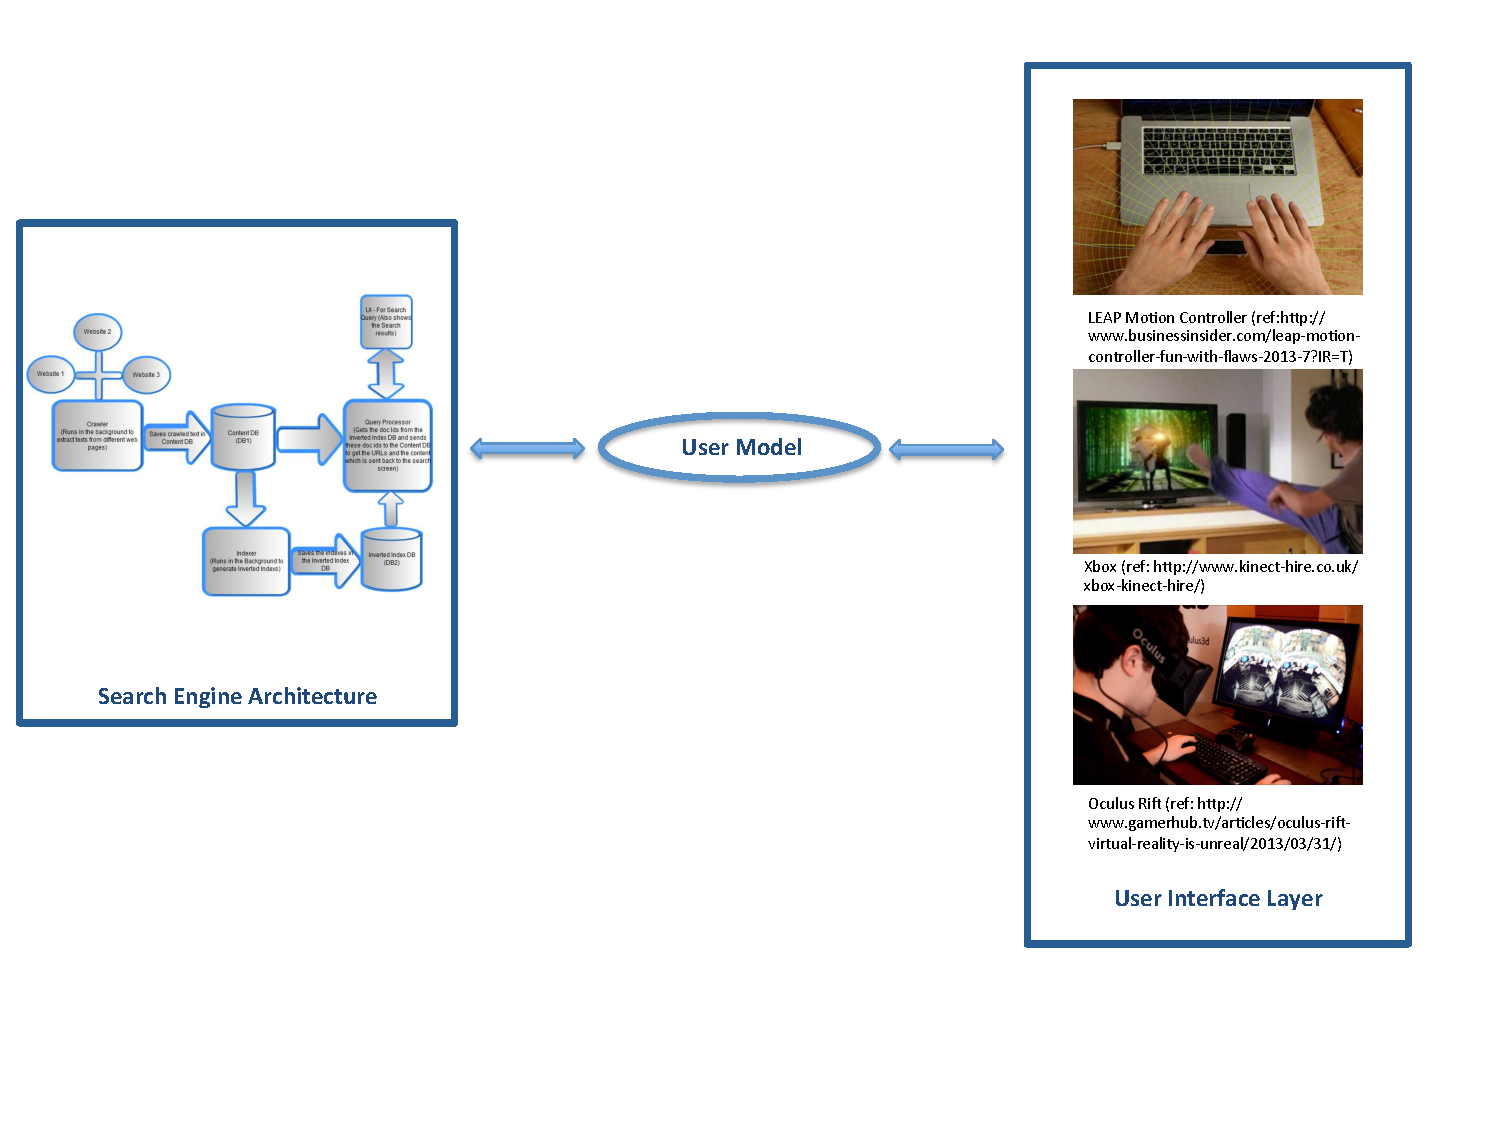
\includegraphics[scale=0.6]{searchEngArchi}\\
Proposed application: The User Model will be applied to existing Search Engine Architecture\cite{seimage}, and be integrated with a Motion Controlled interface.
\end{center}


\subsubsection{Core Features}
\begin{enumerate}
\item  A web application that synthesises the results from three of the largest and most popular search engines (Google, 67.5\%, Microsoft Bing 18.4\% and Yahoo 10.3\%) \cite{adam}

\item The design and implementation of a stereotyped user model of Autism to filter user search results

\item Key Word In Context search; returning verbally-concrete, not text-overloaded results, in a consistent manner. 

\item Prioritisation of results which have first-order semantic relations to the query words (see Section~\ref{the problem}), i.e., they appear in matched context to the search query.

\item Motion controlled UI (see Section \ref{hardware}).
\end{enumerate}

\subsubsection{Non-core Features}
\begin{enumerate}

\item Implement a higher ranking for pages with most images. 
\item Use of WebGL and the three.Js library for 3D UI .
\item Compatibility with other motion controller devices (e.g., head-mounted devices).

\end{enumerate}

\section{Plan for Developing the Solution}

\subsection {Creating a User Model of Autism}\label{usermodel}
\subsubsection{What is a user model?}
A user model is a collection of information associated with a particular user (usually a data structure), with which a system can adapt/customise its behaviour in line with user needs. The information can be gathered when the user 'sign's up' for the service (e.g., Google+, Facebook), and starts the formation of a data model. User modeling has strong implications for human-computer interaction (HCI); by creating a representation of the user, the system can be better informed about how to behave in various circumstances, e.g., the user’s demographics, needs, preferences, likes, dislikes, goals, plans, knowledge, and skill.

\subsubsection{Types of user models}
User models can be static/unchanging (i.e., no algorithms update the model about the changing preferences of the user/ no new information is fed into the model), or dynamic (representation of the user with their up-to-date changes in interests, and interactions with the system). User models may also be stereotyped, where the system infers or assumes characteristics about a user from data gathered from other users within that distinct subset. Lastly a user model can be highly adaptive and model the user on their own, without stereotyping, however this requires a large amount of data before implementation.\\
Stereotyped user models can be built quickly using clusters of characteristics of groups of individuals. Because I will have limited data to work with at the start of the project (only basic information gathered via a registration process), I will build a stereotyped user model of individuals with Autism within Search.

\subsubsection{Adaptive / Personalised Search}
Adaptive or Personalised search associated each user with a HTTP-cookie containing information such as login (gender, age), preferences (languages, interests) and previous search history. This allows the website to ‘remember’ what buttons the user clicked on, or sites visited. This cookie allows the search engine to return results that are highly related to pages that the user visited through previous searches. 

\subsubsection{Disadvantages of Current Adaptive Search for Individuals with Autism}
Although adaptive search seems to have significant user benefit in terms of relevance of returned pages to the user, it decreases the likelihood that the user encounters new information, biasing the results towards the users location and previous site traffic.  This has the unwanted effect of creating a filter bubble \cite{Pariser}, which is argued to close us off from important and relevant information. It creates a personal ecosystem of information for one user, giving the impression that their self interests are all that exist \footnote{The filter bubble also has potential privacy problems, as the user may be unaware that the search has been specifically tailored towards their interests and they wonder why things that they have previously searched for have become more and more relevant. There are search engines that have attempted to address this unwanted effect, by not tracking or saving user information (e.g., DuckDuckGo.com). As users are not linked to their search queries, it limits them being targeted by adverts related to their previous searches.}. Unfortunately the filter bubble may positively reinforce restricted interests in Autism as the user constantly receives feedback about their previous (idiosyncratic and personalized) searches without being able to break out of that repetitive loop. \\Research has suggested personalization also increases ‘background noise’ relative to the search results \cite{briggs}, with a carry-over effect in personalized search, where prior search influences the results from subsequent searches \footnote{It should be noted that personalization of search results generally takes a lower priority for the ranking algorithms than the URLs ranked top in terms of their relevance for the search query.}. This carry-over may be particularly disadvantageous for people with Autism (some of whom already have restricted and repetitive interests) as it muddies their search space.\\
To produce a search tool specifically tailored to reduce the filter bubble effect in Autism, widen the information gateway and reduce the possibility for restricted and repetitive searches, the weighting on previous search results will need to be reduced. This is something I will investigate in the project, particularly for individuals who identify restricted or repetitive interests. For these users, it would limit the possibility that they get trapped in a spiraling loop of ever-narrowing user-relevant information and over-personalization of self-reinforced information ecosystems.

\subsubsection{Persisting the User's Information}
The user will be asked to authenticate a link between their Google+ account and the web application. The Google+ API includes methods to access 4 resource  types; People, their Activities, Comments and Moments. A person is represented with many fields in Google +, including name, gender, title, occupation and so forth. Information about web-search history for any individual user can be obtained from the browser history. 

\subsection{Implementing the Application}\label{api}
\subsubsection{Selecting Search Engines} 
The three most popular search engines (as calculated using an average of the unique monthly visitors) are Google (1,100,000,000), Bing (350.000.000) and Yahoo! (300,000,000)\cite{ebiz}. Google is the goliath question-answering system (query volume = 64.5\%)\cite{adam}, and is often considered the most innovative and dynamic. It is popular amongst users worldwide (using global traffic rank figures, in March 2015). Yahoo (2003) was the first ever web directory service; it has stronger advertising and e-commerce partnerships and has a query volume of 19.8\%. Bing was officially launched in 2005, and has a query volume of 12.8\%, which is substantially less than Google, but nevertheless, is within the top 3 search engines. Other search engines were not included, to limit redundancy of the search results returned (see Section~\ref{Existing Combination/Advanced Search Engines}). 

\subsubsection{APIs, Text-Search Libraries}
I will use API’s provided by Google, Yahoo and Bing. These are more efficient than inspecting the source code for each search-result page (e.g., the Apache Lucene Key Word In Context (KWIC) library is optimised for maximum search efficiency see Section~\ref{apache}). 

\subsubsection{Google Custom Search}
Google Custom Search (GCS) API (available in Java) can be used to create a personalised search engine. GCS requires a domain name and server at configuration, and provides a consumer key and secret, which are hardcoded in the application.\\
Using the API I can extract image search results, page dates, formatting dates, custom snippets, and sort and filter the results. The API alone may not be comprehensive for textual-search (KWIC), and an addional library may be required (see Section~\ref{apache}). Costs \$0.01/search.

\subsubsection{Yahoo BOSS}
To use the Yahoo BOSS Java API, I will create a search engine 'project' to obtain a consumer key and secret. The API offers similar functionality as the GSC, so is not sufficient alone to reach the goals of the project. Costs \$0.01/search.

\subsubsection{Bing Search API (Data)}
The Bing Search API can produce results for Web, Images, News, Videos, Related Search. It also includes spelling suggestions based on the query entered. Costs \$0.00/search (max 5000 searches/month)

\subsubsection{Faroo API}
Faroo is a free (Java) API, claiming to combine Google, Yahoo and Bing. Faroo can return news search, trending pages, and can sort results \cite{faroo}. However, as it only offers Web Search from 2 billion pages it has indexed (compared to Google: 46.7 billion \cite{websize}), it is not comprehensive enough for the current project.

\subsubsection{Apache Lucene Library}\label{apache}
Apache Lucene Library is a text-search library (written in Java), and provides powerful, scalable, accurate and efficient algorithms to search textual data. The API offers the possibility to carry out phrase, wildcard, proximity and range queries. The library also affords ranked searches, with type tolerant suggesters and field searching.

\subsubsection{Key Word In Context} \label{KWIC} 
The Apache library also allows contextual-text search, also known as Key Word In Context (KWIC)\cite{kwic}. KWIC works by forming an index to allow each word to be searchable. The library takes care of the efficiency of this process, and can return weighted terms of a given query (as an example).


\subsubsection{Google+ API}
A user will first authenticate their personal Google+ user profile with the web application being developed, and these data (including age, gender, lifestyle, frequent tasks, tools/resources commonly used) will therefore be acccessible via the API (available in Java)\footnote{It is also be possible to store information in the 'about me' section on the profile about individual diagnosis (Autism, Asperger, and high/low functioning). This information can be parsed when the query is submitted to the search engine.}. 

\subsubsection{API for 'LEAP' Motion Controller}
LEAP Motion SDK offers an API to get tracking data from the LEAP Motion Service. A WebSocket interface, allows LEAP Web Based applications, and a WebSocket server listening in on http://127.0.0.1:6437\footnote{The user can enable or disable the WebSocket server as they choose to do so, in the device's control panel.}.
The server sends tracking data in JSON messages and an application can send configuration messages back. This library will be used to establish connection to the server and consume the JSON messages \cite{leap}. 


\subsubsection{ThreeJs Library (Non-Core)}
This Javascript library enables WebGL-3D in a web browser. WebGL brings hardware-accelerated 3D graphics to the browser without installing additional software. This library may be used to better integrate the application with the motion controller, and improve the experience of embodiment, UX, and UI of the application.


\subsection{Integrating the Application with Motion Controller Hardware }\label{hardware}
\subsubsection{Hardware Selection Process}
Two options were available; the Oculus Rift Virtual Reality head mounted display, and, the LEAP motion controller. The hardware was selected as follows: 
\begin{enumerate}
\item Accurate timing of the device correlates a good UX. The LEAP has options to ‘poll’ frames at a constant rate (to keep timing of movement accurate).
\item Cognitive ‘lag’ time. Each of our senses operates with a different lag time. Hearing has the fastest sense-to-cognition/understanding time; sight is the slowest. The device should therefore work with the combinatorial configuration of the senses.
\item As this is a tool to be used with individuals with Autism, the sensory experience (imposition) of the device cannot be overwhelming.
\item Cognitive-load should not be high (operating the device should not require a great deal of cognitive effort).
\item The device should integrate with concrete behaviours, e.g., drop or grab. 
\item Affordability for users.
\end{enumerate}
The two main reasons to persue the LEAP before the Oculus VR were, (1) it's non-imposing nature (no head mount), and (2), the affordability of the controller.

\subsubsection{LEAP Controller}
The LEAP can recognize and track hands, fingers, finger-like tools, positions, motions and gestures using infrared light and optical sensors along the x, y and z axes (cartesian coordinate system). The controller has a 150-degree field of view, and can operate in a range of 1 inch to 2 feet. The API works with distance in millimetre resolution. Time is measured in microseconds, speed in mm/s and angles in radians.

\begin{center}
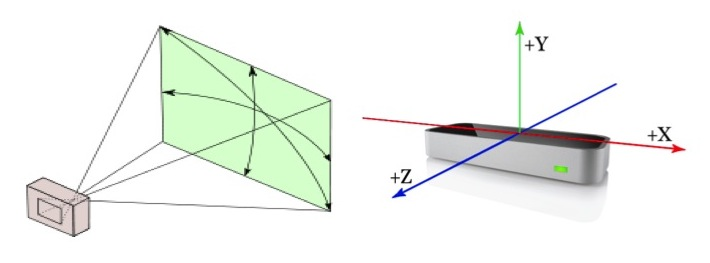
\includegraphics[scale=0.4]{leap}\\
The LEAP controller, with 150 degree view \cite{leap}.
\end{center}

The LEAP uses frames to represent tracked entities such as hands, fingers, tools or gestures. Motion data is recorded as a set of frames (stored, read-only) containing the detected information. Frames can be created by calling the Controller.frame(). Up to 60 can be held in the history buffer. Frames may be 'dropped' if there are resource contrainsts, or, they are missed.

\subsubsection{Hands}
The Hand class, returns information about the position of fingers, and arm (left/right).

\begin{center}
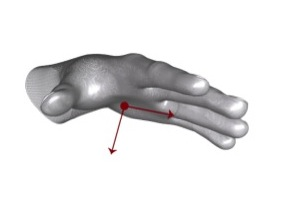
\includegraphics[scale=0.4]{palm}\\
The Hand palmNormal() method and direction vectors define the orientation of the hand \cite{leap}.
\end{center}

The software uses parts of visible hands, internal models and previous observations to form a model of the hand. There is a Hand.confidence() method that provides a rating of how well the observed data fit the internal model \cite{leap}.

\subsubsection{Arms}
The Arms class can return information about orientation, length, width and end points of movements. The LEAP controller software bases these return measurements on previous observations of the user, and using typical human proportions.

\subsubsection{Fingers}
These characteristics are based on the anatomy of the hand, and recent observations. 

\begin{center}
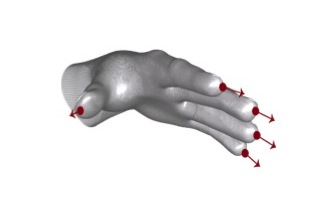
\includegraphics[scale=0.4]{fingers}\\
Finger tip position and direction are given as vectors. \cite{leap}.
\end{center}


\subsubsection{Tools \& Pointables}
Tools can represent any real object (noun), but are longer, straighter and thinner than fingers. Tools must be cylindrical.

\subsubsection{Gestures}
The LEAP recognises certain movement patterns (CircleGesture, KeyTapGesture, ScreenTapGesture and SwipeGestures) allowing the user to indicate an intent.


\subsection{Project Plan}\label{plan}

\subsubsection{Project Timeline}
The start date of the project is June 5th 2015, and end date is September 13th 2015. 
\begin{table}[h]
\caption{Project Stages} 
\centering
\begin{tabular}{ L |c| L}
\hline\hline 
Dates & Task & Priority\\ [0.5ex]
\hline 
Jun 05 - Jun 12 & Configure relevant API's \& Libraries to domain name/server & MUST\\
\hline 
Jun 13 - Jun 19 & Synthesise search results & MUST\\
\hline 
Jun 20 - Jun 27 & Research \& build user (and data) model of Autism & MUST\\
\hline 
Jun 28 - Jul 06 & Work on configuration with Google+ API & MUST\\
\hline 
Jul 07 - Jul 14 & Apply user model to Search& MUST\\ 
\hline 
Jul 14 - Jul 21 & Develop UI & MUST\\
\hline 
Jul 21 - Jul 28 & Integrate motion controller tools& MUST\\
\hline 
Jul 29 - Aug 05 & Develop questionnaire and eye-tracker set up & MUST\\ 
\hline 
Aug 06 - Aug 13 & Test the model and ask for user feedback & MUST\\
\hline 
Aug 14 - Aug 21 & Revise the user model and UI & MUST\\
\hline 
Aug 14 - Aug 21 & Develop UI with other motion controllers & COULD\\
\hline 
Aug 22 - Aug 29 & Develop UI using WebGL/threeJs library & COULD\\
\hline 
Aug 22 - Aug 29 & Write up project report & MUST\\ 
\hline 
Early Sep (tbc) & Present findings to supervisor & MUST\\
\hline 
Sep 13 & Submit report & MUST\\[0.5ex]
\hline
\end{tabular}
\label{stages} 
\end{table}

\subsubsection{Methodology}
There is a relatively short deadline in which a single developer will research and deliver a system prototype and report. The APIs, technology and areas of development are unfamiliar. As the final product depends on user feedback testing, there is an element of uncertainty about what the final product will be/should look like. These characteristics suggest that the most suitable methodology to deliver the application is an Agile-like Methodology. I will focus on early development and rapid feedback to make adjustments to the project's direction. This methodology offers the most flexibility and adaptability.


\subsubsection{Development Languages}
The Google, Yahoo, Bing and Apache Lucene APIs are available in Java. The LEAP SDK sends Frame information in JSON format to Web Browsers. As a non-core feature, I may use a 3D interface with the three.Js library which is also JSON format. I will use HTML5 for the development of the aesthetics of the Web Application itself.
For testing I will use JUnit, JSON Test and Mockito (for user/external dependencies).\\
JSON is light weight, language-independent data format, and a good tool for sharing data. Importantly JSON offers faster execution and server-side parsing by storing the data in arrays, so that the transfer of data is faster. Faster parsing is particularly important for sharing the LEAP motion controller data. Some of the drawbacks of JSON are that it only has limited support tools available, and little error handling capabilities. It is also vulnerable as it returns responses in wrapped function calls which are vulnerable to attack. Java is a platform and operating-system independent language. It offers a simple, dynamic, robust object oriented, and functional language. There is excellent documentation available for the language, with many third party, open source libraries.\\
I will use Eclipse text editor and attempt to make the application compatible with Google Chrome browser (as it is WebGL-compatible and useful for 3D interfaces). I will use Git for Version Control.

\subsubsection{Testing}
\subsubsection{User Testing}
I will test the application with a group of individuals with Autism. I will
\begin{enumerate}
\item Invite adolescents and adults Autism to use the web application.
\item Obtain their feedback (relevance/explicit feedback, and, implicit feedback, e.g., 'clicks'). 
\item Design a questionnaire to gather qualitative data. 
\item If time allows, I will use the Tobii Eye-tracker TX300 (Department of Psychology, Birkbeck University of London) to gather high resolution eye-tracking data as users test the application. 
\item Revise the model and ideas. Choosing the best possible approach/tools to achieve optimization for this group of individuals.
\end{enumerate}

\subsubsection{Unit Testing}
I will be implementing Test Driven Development (TDD)\footnote{The TDD process involves iterating through the write-test-then-write-code process. First writing a test for some functionality, and second, writing just enough production code to make the test pass.} with JUnit (version 4.12), and where there are external dependencies, these will be mock tested using Mockito \footnote{mockito.org}. JSON Test will be used to test JavaScript Object Notation \cite{jsontest}. I will run both unit and regression tests.

\subsubsection{Risks/issues, probabilities and mitigation of impact}
The risks associated with the project, their impact and how I will mitigate them, is outlined in~Table \ref{risks}. 
\begin{table}[H]
\caption{Risks \& Impact Mitigation} 
\centering
\begin{tabular}{|c | c | p{5cm} | p{5cm} |}
\hline\hline 
Liklihood & Impact & Risk & Mitigation\\ [0.5ex]
\hline 
LOW & HIGH & API's require significantly high payment & Find/use alternative\\
\hline 
LOW & HIGH & KWIC library does not offer methods needed to achieve goals of contextual text search & See if I can implement the method, or find additional API\\
\hline 
LOW & MEDIUM & Cannot get research participants with Autism to take part in a usability test & Expand age range of interest in attempt to find participants\\ 
\hline 
MEDIUM & MEDIUM & Google+ API does not configure a user persona/user model well & Use Facebook or alternative\\
\hline 
MEDIUM & HIGH & LEAP does not integrate with web application & Investigate user forums, contact LEAP to source answers, adjust web application accordingly.\\
\hline
MEDIUM & HIGH & User Model lacks power and users are unhappy with the Search system & Gather feedback for a further iteration. Modify weights of parameters in the algorithm. Revise the model. \\
\hline
MEDIUM & HIGH & Not enough turn around time to implement the feedback & Develop plan and prototype in time for report submission\\[1ex]
\hline
\end{tabular}
\label{risks} 
\end{table}

\subsection{Summary \& Concluding Statement}\label{future}
I have proposed to research and build a User Model within Search for people with Autism. I describe a model (based on well-understood aspects of cognition in Autism) to apply to search results, using text and content based libraries which will refine search results for these individuals. I hope these insights will assist with the forthcoming information-overload problem by exploiting these user models to turn the masses of information available into a specific set of “information goods”. 

\begin{thebibliography}{100}

\bibitem {gameshealth} Games for Health (2012) \textit{Screen-based technologies and Autism. 1}: 248-53

\bibitem {usermodel}Shen, X., Tan, B. and Zhai, C. (2005) Implicit User Modeling for Personalized Search, \textit{Conference on Information and Knowledge Management}, Bremen, Germany.

\bibitem{motioncontrollerforautism} Garzotto, F., Valoriani, M. and Bartoli, L. (2014), Touchless Motion-Based Interaction for Therapy of Autistic Children, Virtual, Augmented Reality and Serious Games for Healthcare, \textit{Intelligent Systems Reference Library, 68}, 2014, pp 471-494

\bibitem{moore}Moore, D. J., McGrath, P., \& Thorpe, J. (2000). Computer aided learning for people with autism—a framework for research and development. \textit{Innovations in Education and Training International, 37}, 218–228.

\bibitem{workingmem}Baddeley, A.D., \& Hitch, G. (1974). Working memory. In G.H. Bower (Ed.), \textit{The psychology of learning and motivation: Advances in research and theory, 8}, 47–89. New York: Academic Press.

\bibitem{leap} Leap Motion, \textit{Java SDK Documentation}, \\https://developer.leapmotion.com/documentation/java/index.html Retrieved 1 April 2015.

\bibitem{briggs}Briggs, J. \textit{A Better Understanding of Personalized Search}. https://www.briggsby.com/better-understanding-personalized-search/, Retrieved 5 April 2015.

\bibitem {Brusilovsky} Brusilovsky, P. and Tasso, C. (2004) User modeling for Web information retrieval. \textit{User Modeling and User Adapted Interaction, 14}, 2-3, 147-157.


\bibitem {CDC}Developmental Disabilities Monitoring Network Surveillance (2010) \textit{Centers for Disease Control and Prevention (CDC). Prevalence of autism spectrum disorders: Autism and Developmental Disabilities Monitoring Network, United States. MMWR Surveill Summ.2009; 58}, 10:1–20


\bibitem {Shane and Albert}Shane, H. C. and Albert, P. D. (2008) Electronic screen media for persons with autism spectrum disorders: results of a survey. \textit{Journal of Autism Developmental Disorders, 38},8 :1499-508. doi: 10.1007/s10803-007-0527-5.

\bibitem{jsontest}jsontest \textit{JSON Test}, http://www.jsontest.com/, Retrieved 8 April 2015.

\bibitem{triad}National Autistic Society, \textit{The Autistic Spectrum}, \\http://media.kingdown.wilts.sch.uk/mod/page/view.php?id=7374, Retrieved 20 March 2015

\bibitem {Lasater}Lasater, M. W., \& Brady, M. P. (1995). Effects of video self-modeling and feedback on task fluency: A home-based intervention. \textit{Education and treatment of children, 18}, 389-407.

\bibitem {Pariser} Pariser, E (2011) First Monday: What's on tap this month on TV and in movies and books, \textit{The Filter Bubble by Eli Pariser}. USA Today. Retrieved April 7, 2015. 

\bibitem{fabienne}Fabienne Samson, Laurent Mottron, Isabelle Soulières, Thomas A. Zeffiro (2011). Enhanced visual functioning in autism: An ALE meta-analysis. \textit{Human Brain Mapping} DOI: 10.1002/hbm.21307

\bibitem{kwic}Manning, C. D., Schütze, H. (1999) \textit{Foundations of Statistical Natural Language Processing}, p.35. The MIT Press.

\bibitem{attention} Bronwyn, M, Murray, M, and Durkin, K. (2003) Weak central coherence, poor joint attention, and low verbal ability: Independent deficits in early autism. \textit{Developmental Psychology, 39}, (4), 646-656. http://dx.doi.org/10.1037/0012-1649.39.4.646

\bibitem{disengagement}
Elsabbagh, M., Volein, A., Holmboe, K., Tucker, L., Csibra, G., Baron-Cohen, S., Bolton, P., Charman, T., Baird, G. and Johnson, M. H. (2009), Visual orienting in the early broader autism phenotype: disengagement and facilitation. \textit{Journal of Child Psychology and Psychiatry, 50}, 637–642. doi: 10.1111/j.1469-7610.2008.02051.x

\bibitem{seimage} Pray, S. \textit{Inverted Index : The basic ingredient behind the recipe called Search Engine}https://insightsdelight.wordpress.com/2012/01/24/inverted-index-the-basic-ingredient-behind-the-recipe-called-search-engine/, Retrieved 8 April 2015

\bibitem {Economist} Pariser, E. (2011) \textit{Invisible sieve: Hidden, specially for you}. The Economist. Retrieved April 8, 2015. Mr 

\bibitem {MacDuff} MacDuff, Krantz, \& McClannahan (2001). Prompts and prompt-fading strategies for people with autism. In C. Maurice, \& G. Green (Eds.), \textit{Making a difference: Behavioral intervention for autism}, 37-50. Austin, TX: Pro-Ed.

\bibitem{websize} Kunder, M. D. \textit{The size of the World Wide Web: Estimated size of Google's index}, http://www.worldwidewebsize.com/, Retrieved 8 April 2015.


\bibitem {Sherer}Sherer, M., Pierce, K. L., Paredes, S., Kisacky, K. L., Ingersoll, B., Schriebman, L. (2001). Enhancing conversation skills in children with autism via video technology. \textit{Behavior Modification, 25}, 140-158.


\bibitem {Thiemann}Thiemann, K. S., \& Goldstein, H. (2001). Social stories, written text cues, and video feedback: Effects on social communication of children with autism. \textit{Journal of Applied Behavior Analysis, 34}, 425-446.

\bibitem{ebiz}eBizMBA inc, \textit{The eBusiness Guide}, www.eBizMBA.com; Retrieved 20 March 2015

\bibitem {Google}Sullivan, D. \textit{Google Still World’s Most Popular Search Engine By Far, But Share Of Unique Searchers Dips Slightly},  http://searchengineland.com/google-worlds-most-popular-search-engine-148089, Retrieved 20 March 2015.  

\bibitem {Vaishnavi1}Sandeep Vaishnavi1 , Jesse Calhou , and Anjan Chatterjee (2001). Binding Personal and Peripersonal Space: Evidence from Tactile Extinction. \textit{Journal of Cognitive Neuroscience 13}, 2, pp. 181–189

\bibitem {adam}Lella, A., (2014). comScore Releases March 2014 U.S. Search Engine Rankings. ComScore.com. Retrieved 21 Feb 2015

\bibitem{bowler}Dermot M. Bowler, Sebastian B. Gaigg, John M. Gardiner (2014) Binding of Multiple Features in Memory by High-Functioning Adults with Autism Spectrum Disorder, \textit{Journal of Autism and Developmental Disorders September 2014, 44}, Issue 9, pp 2355-2362

\bibitem {googlebing} Parrack, D.\textit{4 Search Engines That Combine Google \& Bing}, http://www.makeuseof.com/tag/4-search-engines-that-combine-google-bing/, Retrieved 6 April 2015.


\bibitem{faroo}Faroo, \textit{Free Faroo API}, http://www.faroo.com/hp/api/api.html, Retrieved 6 April 2015.

\bibitem{mottron} Laurent Mottron, Jacob A. Burack, Johannes E. A. Stauder, Philippe Robaey (1999) Perceptual Processing among High-functioning Persons with Autism. \textit{Journal of Child Psychology and Psychiatry 40}, (2), 203–211. doi:10.1111/1469-7610.00433

\end{thebibliography}
\end{document}
